begin{figure}[h!]
    \hspace{-1.5em}
    \begin{subfigure}{0.5\textwidth}
    \centering
    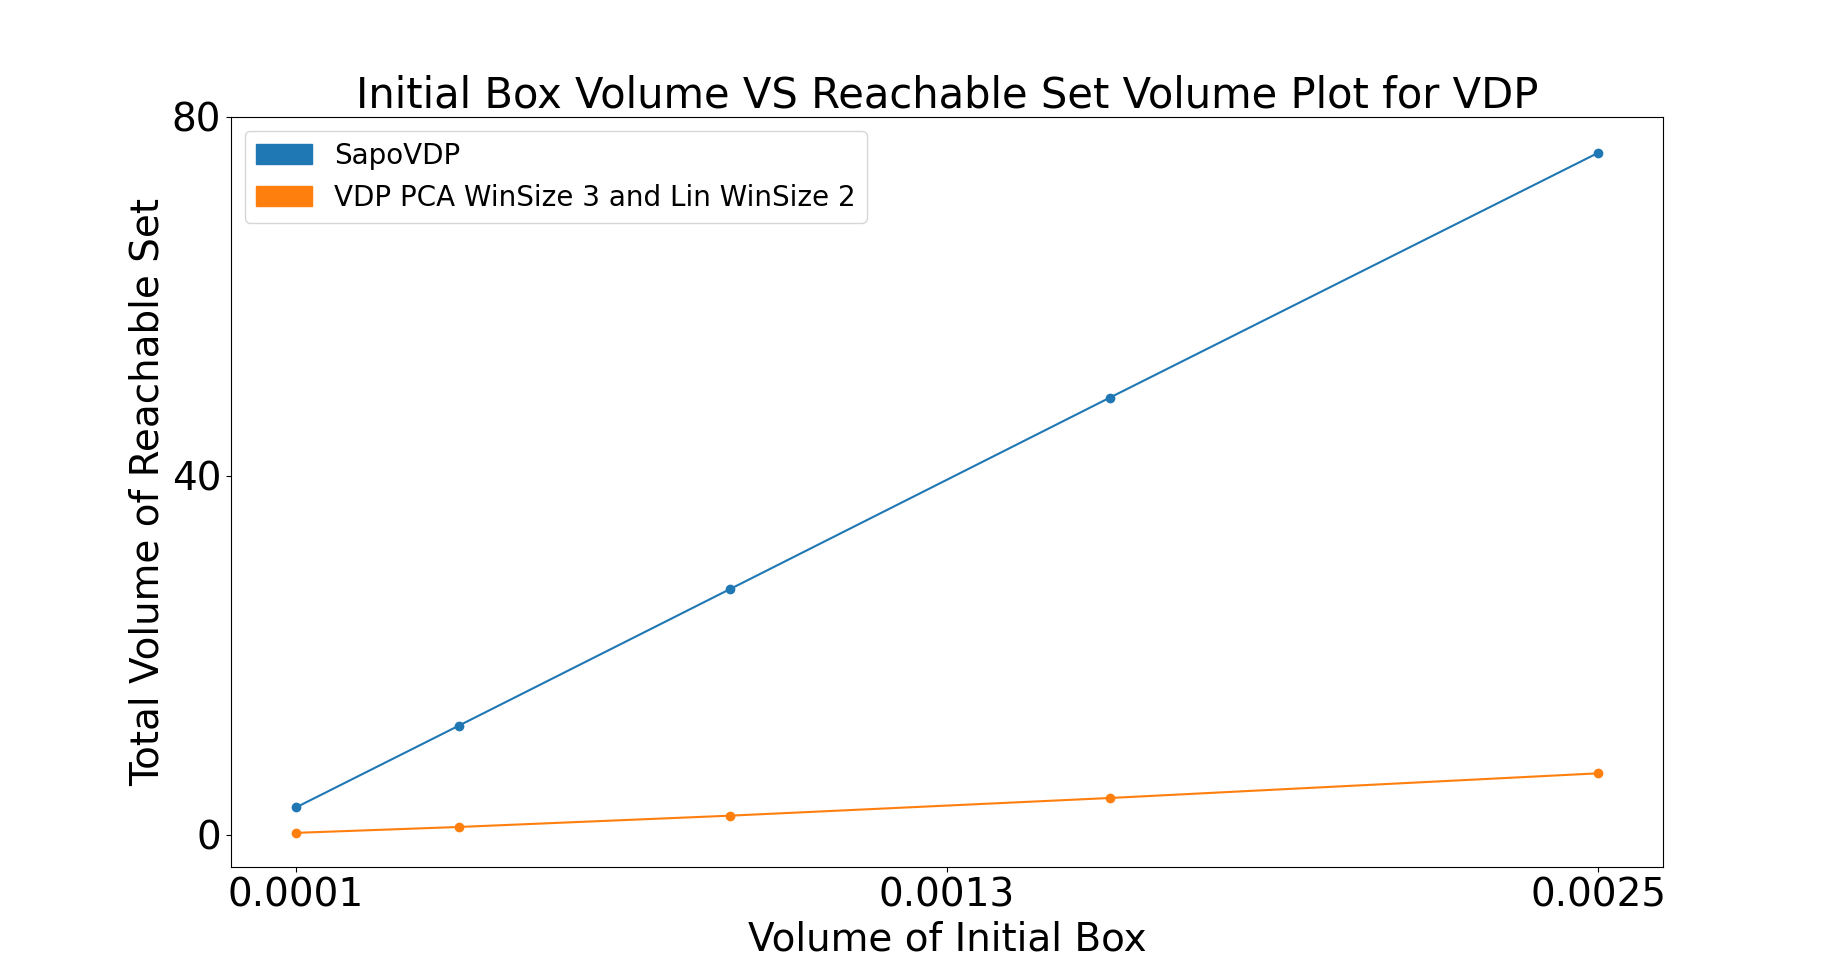
\includegraphics[width=1.1\textwidth, height=0.75\textwidth]{figures/InitVolVSReachVol/VDPInitReachVol.png}
    \caption{Vanderpol}
    \end{subfigure}%
    %\hspace{1em}
    \begin{subfigure}{0.5\textwidth}
    \centering
    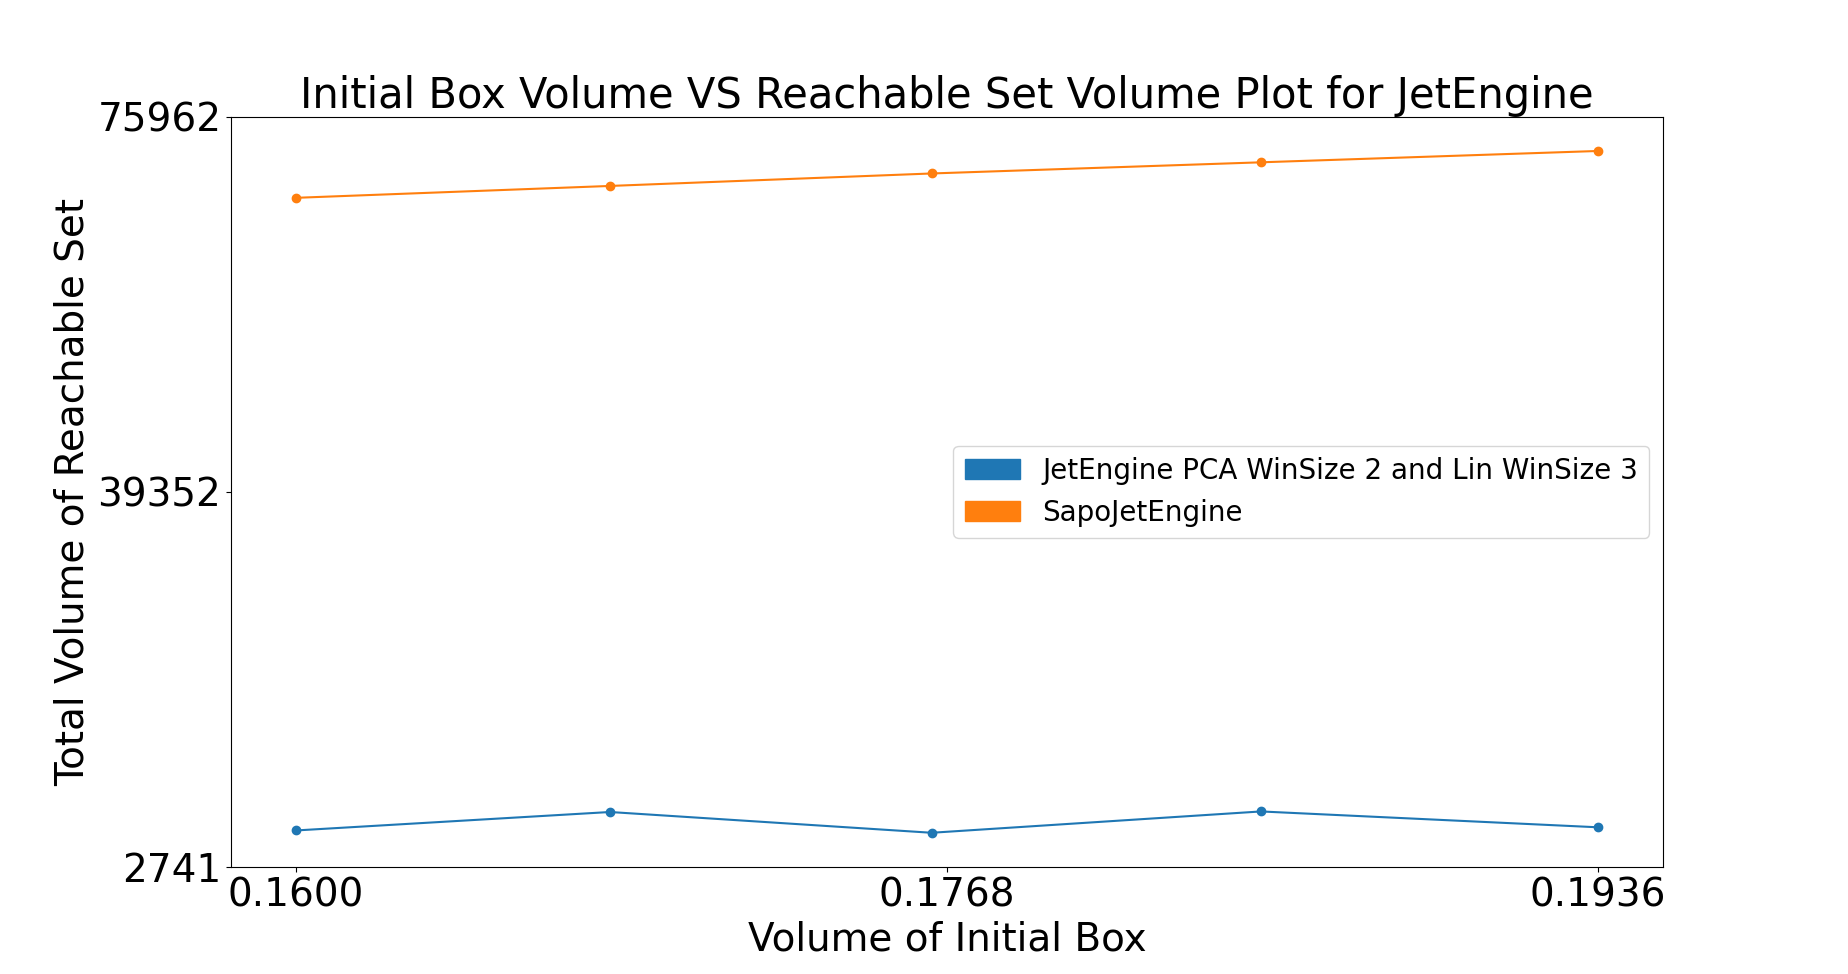
\includegraphics[width=1.1\textwidth, height=0.75\textwidth]{figures/InitVolVSReachVol/JetEngineInitReachVol.png}
    \caption{Jet Engine}
    \end{subfigure}

    \hspace{-1.5em}
    \begin{subfigure}{0.5\textwidth}
    \centering
    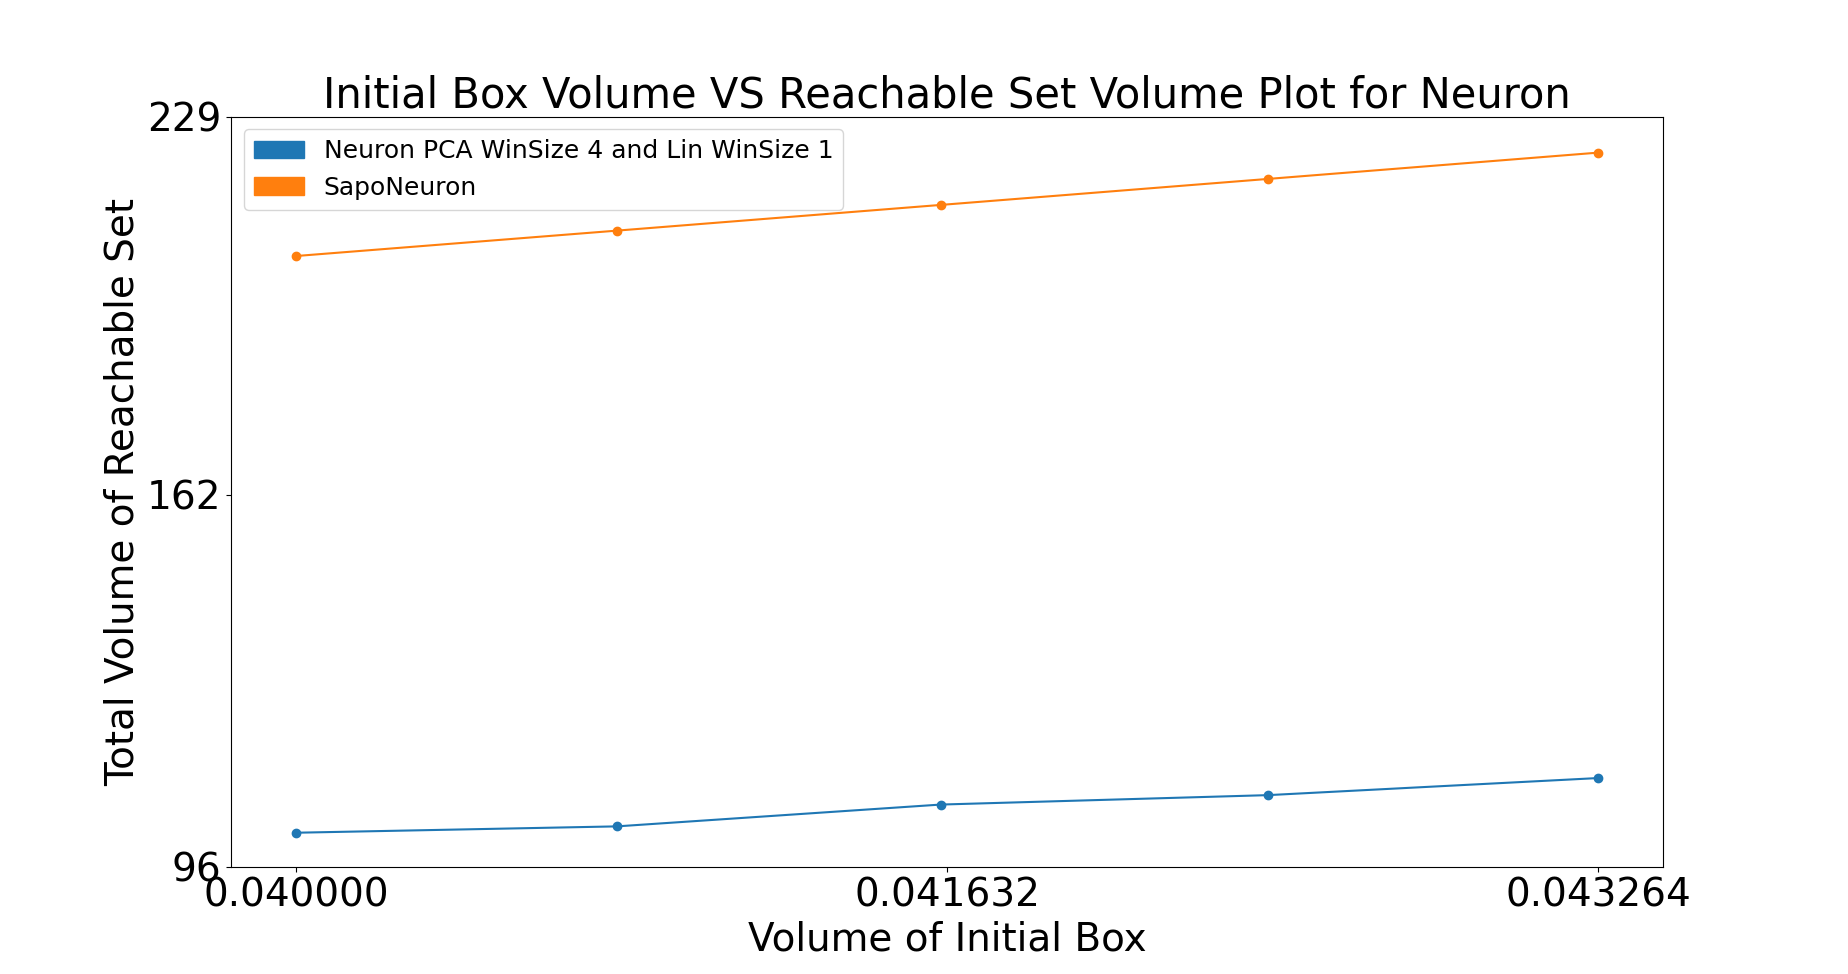
\includegraphics[width=1.1\textwidth, height=0.75\textwidth]{figures/InitVolVSReachVol/NeuronInitReachVol200steps.png}
    \caption{Neuron}
    \end{subfigure}%
    %\hspace{1em}
    \begin{subfigure}{0.5\textwidth}
    \centering
    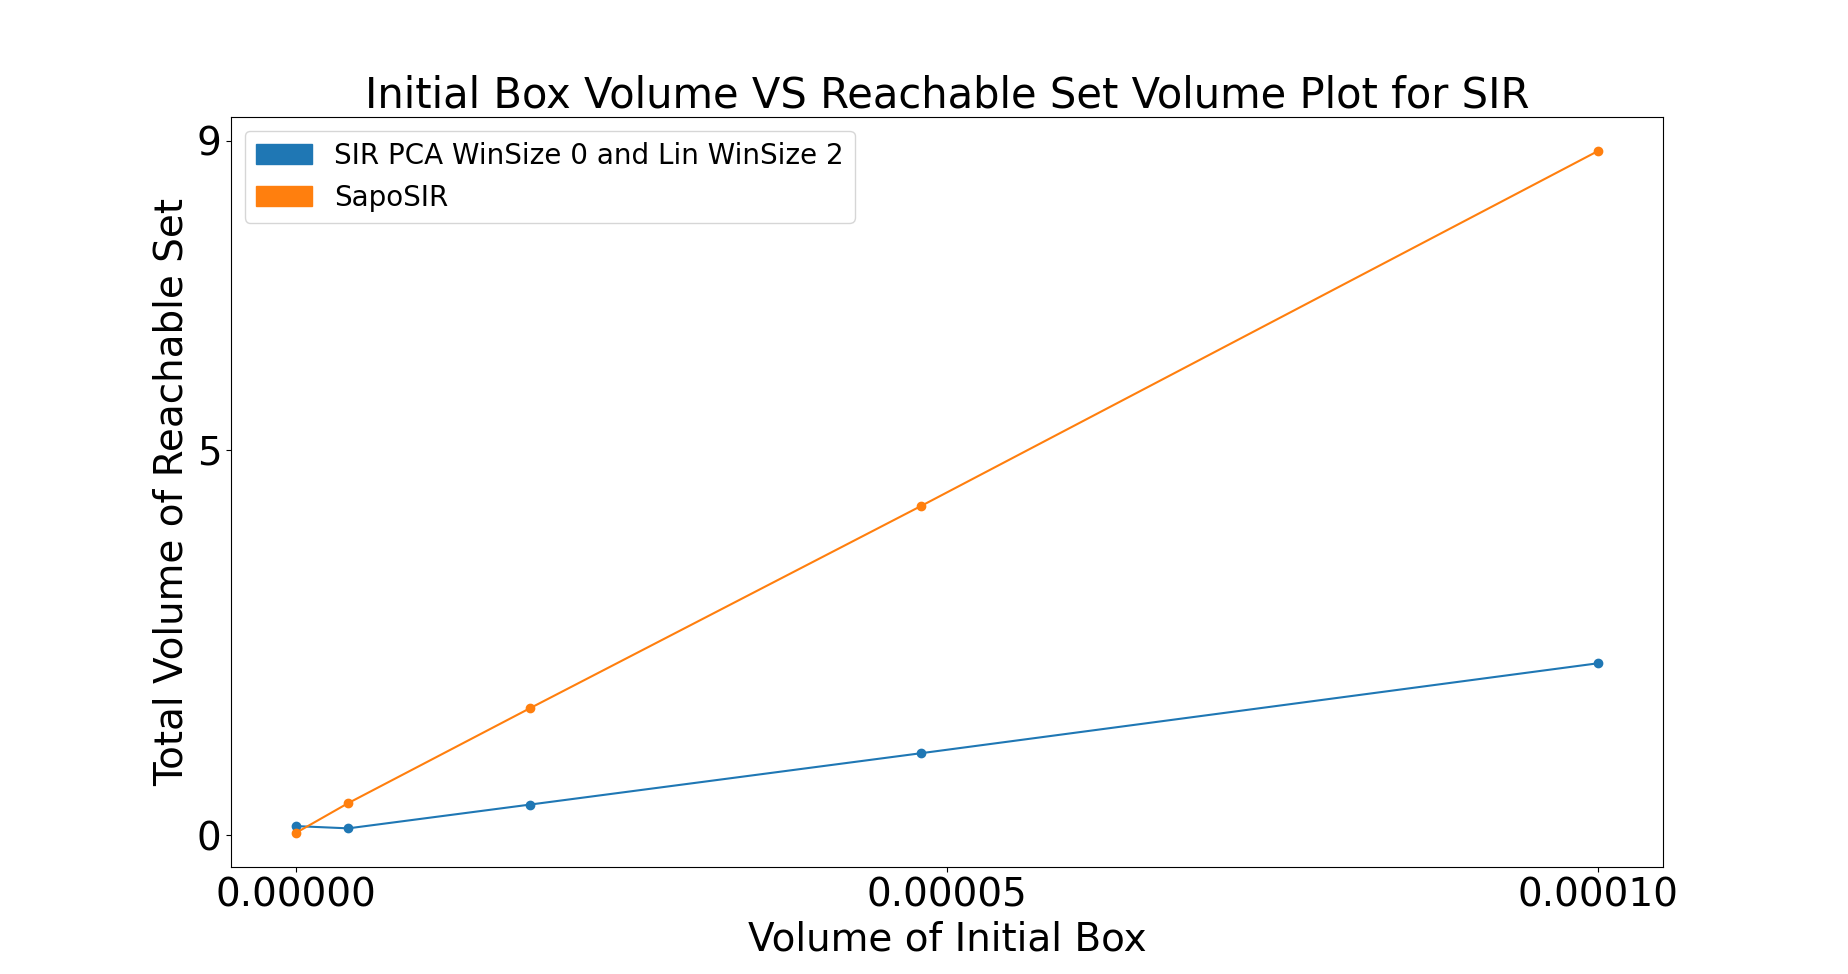
\includegraphics[width=1.1\textwidth, height=0.75\textwidth]{figures/InitVolVSReachVol/SIRInitReachVol.png}
    \caption{SIR}
    \end{subfigure}

    \hspace{-1.5em}
    \begin{subfigure}{0.5\textwidth}
    \centering
    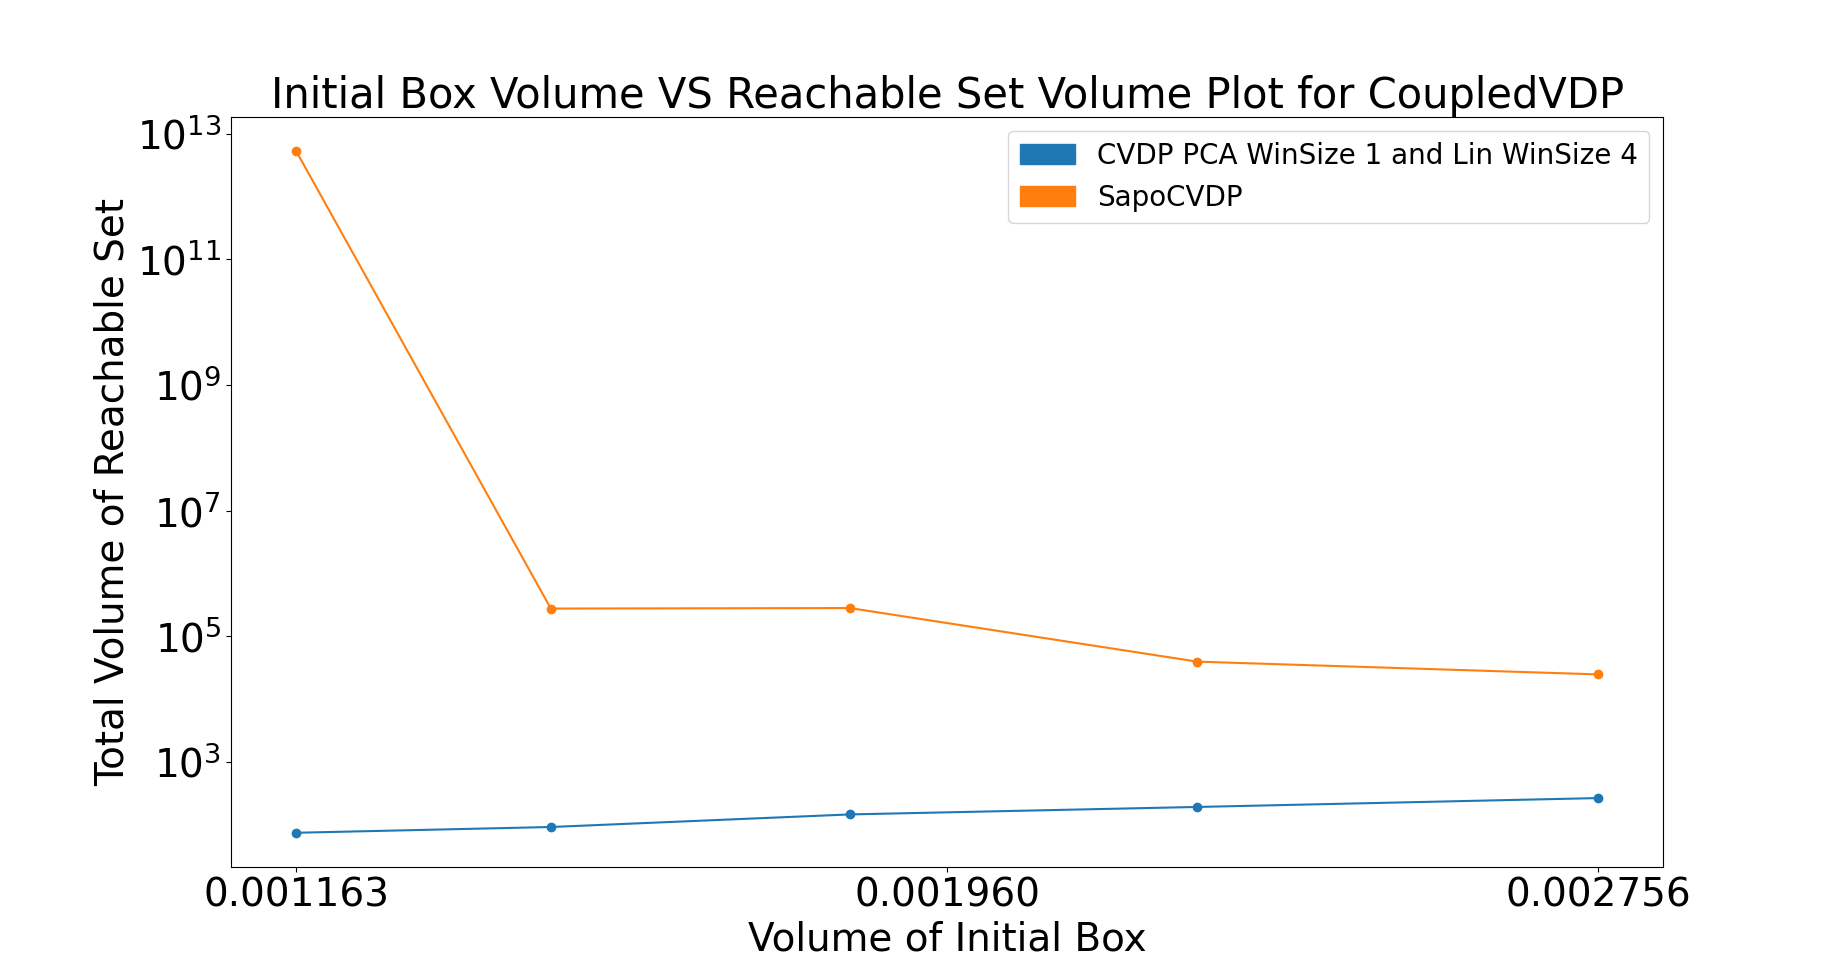
\includegraphics[width=1.1\textwidth, height=0.75\textwidth]{figures/InitVolVSReachVol/CVDPInitReachVol.png}
    \caption{Coupled Vanderpol}
    \end{subfigure}%
    %\hspace{1em}
    \begin{subfigure}{0.5\textwidth}
    \centering
    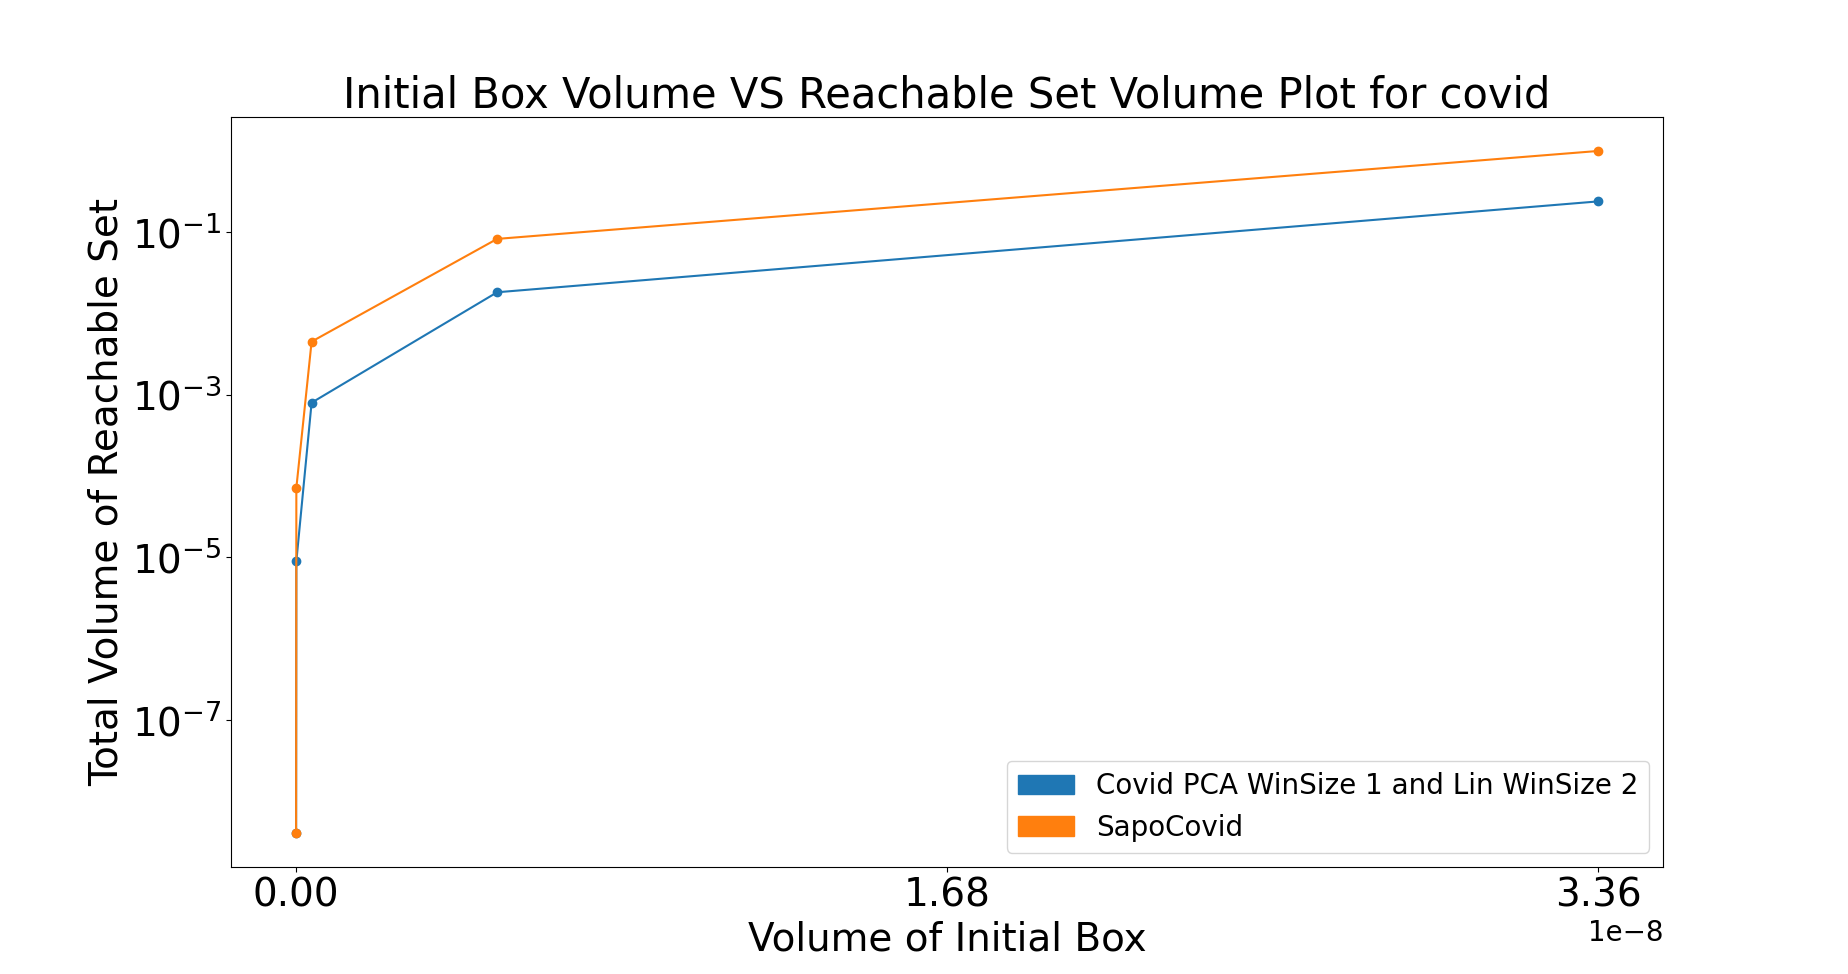
\includegraphics[width=1.1\textwidth, height=0.75\textwidth]{figures/InitVolVSReachVol/CovidInitReachVol.png}
    \caption{COVID}
    \end{subfigure}

    \caption{Comparison between the performance of diagonal static parallelotope bundles and that of the best performing dynamic parallelotope bundles as the volume of the initial set grows.}
    \label{fig:InitVolReachComp}
\end{figure}
\clearpage
